\chapter{Sea Level Rise and Subsidence}
\chapterauthor{Luyi Huang and Betel Solomon Tesfamariam\footnote{Statement of Contributions: }}



\section{Introduction}
  Since the large-scale industrialization of Europe in the late 20th century, increased pollution levels and subsequent anthropogenic climate change has become a cause for concern for many people around the world, as well in the science domains. Since 1988, the Intergovernmental Panel on Climate Change (IPCC), set up by the World Meteorological Organization (WMO) and the United Nations Environmental Program, has been collating scientific research on the factors and impacts of climate change in order to design response strategies to be included in international conventions on climate. However, these strategies rely on international cooperation and national compliance. One of the consequences of climate change is sea-level rise, and recent research calls attention to the instability of the Greenland and West Antarctic ice sheets as a factor that may result in a 1m increase in sea-levels in the 21st century (Nicholls et al., 2010). Nicholls et al. (2010) examine the impact of sea-level rise in a the present-day global context whereby there is no mitigation policy and the global mean near-surface temperature could possibly reach 4 degrees celsius by 2100.
  
  Sea level rise is commonly known as a global climate change event which has taken place for thousand of years as a result of changes in tectonic plates and consequent subsidence and uplift of  land. It has been predicted to continue for centuries. However, certain locations will experience more or less sea level change due to the combined stratigraphic activities, resulting in local residents being impacted to different extents. Coastal and island residences are considerably being put in risk of coastal erosion, salt water intrusion, flooding and potential loss of habitats. Some questions we raise in this chapter include what contributes to global as well as local sea level rise?  Yet looking a local perspective, what are the effects brought to local farmers in Southeast Asia?
  
 Countries in Southeast Asia are especially vulnerable to global climate change because of (i) their long costalines, (ii) high concentration of human and economic activities in coastal areas, (iii) large and growing populations, and (iv) the importance of agriculture as a source of employment and income (ADB 2009).  Southeast Asia is at risk of being negatively impacted by climate change over the next 20 years due to the region's large and growing  population, long coastlines, abundant low-lying areas, reliance on the agricultural sector, and dependence upon natural resources. In order to understand how current sea levels around the world are changing it is useful to consider the historical context of sea level rise. This chapter will begin by providing an overview of how national governments and international organizations have responded to the reality of sea level rise and the challenges it poses for people living in coastal zones. Following this, a discussion of how sea level rise has impacted and continues to impact Southeast Asia will be offered, providing an introduction to the specific impacts of sea level rise in the Vietnamese Mekong Delta. The role that carbon dioxide plays in causing sea level rise will also be discussed in order to present how natural occurrences can be exacerbated by anthropogenic activity. This chapter will also present how the geological formation of Southeast Asia has historically affected sea level rise, which will lead into a discussion of the impact of isostasy on sea level rise, another mechanism that is influenced by human activities.
 
The case study of the Vietnamese Mekong Delta (VMD) is presented towards the end of the chapter to illustrate how the geographical and geological characteristics of the VMD inform our understanding of why this region is vulnerable to sea level rise. 
  This will be followed by a discussion of the processes that lead to delta formation. Natural spaces and processes are however influenced by the political decisions of humans and therefore the socio-economic and political context of the VMD will be discussed. Groundwater extraction in the VMD and dam construction in the Mekong River, two anthropogenic activities that influence how sea-level rise impacts the VMD, will be discussed in depth to reveal the ways in which transnational politics, arsenic contamination and subsidence determine the threats posed by sea level rise and how they will be mitigated.
  
Small islands in and around Africa, Southeast, and east Asia are identified as being the most vulnerable regions to rising sea level. Coastal adaptation is a systemic process but the increased exposure to sea level rise in these regions is not being countered by a high adaptive capacity. The violent conditions of the transactional interactions between the global north and the global south result in manifestations of slow violence such as a disproportionate impact of climate change in the global south, which include the most vulnerable regions which are identified by Nicholls (2010).  


\section{Sea Level Rise in Southeast Asia}
\subsection{Southeast Asia Geography}

  Maps have proven to be an important analytic as well as informative source for environmental and climate research. While maps are generally perceived as an impersonal type of knowledge, they tend to ``dessocialize'' the territory they represent \citep{harley2009maps}. The boundaries defined in maps can differ depending on a wide range of factors related to social, political and economic characteristics of the regions being studied. Especially under colonial influence, the connections between maps, power and knowledge are enhancing in political geography. The practical actions undertaken with maps: warfare, boundary making, propaganda, or the preservation of law and order, are documented throughout the history of maps \citep{harley2009maps}. Therefore while we introduce the physical and geological boundary of Southeast Asia and present maps later on in this chapter, we wanted to inform readers to be cautious and thoughtful of the process and implication of map making. 

The geographical region of Southeast Asia is commonly described as a corner of the Asian continent consisting of regions east of the Indian and south of China (Figure. 1). Geographically, the region is categorized into two subregions: Indochina (the mainland Southeast Asia) and Malay Archipelago (Maritime Southeast Asia) between Pacific Ocean and Indian Ocean. Generally nations fall under Southeast Asia include but not restrain: Cambodia, Lao, Burma, Malaysia, Thailand, Vietnam, Indonesia, Philippines, Singapore, and Burnei. The region is located near the intersection of geological plates, with frequent tectonic and volcanic activities. The outer boundary of Southeast Asia is an arc formed by the islands of Indonesia and the Philippines, and area of active subduction that manifests itself in frequent earthquakes, occasional tsunamis and periodic volcanic eruptions. The inner mainland part of the region was shaped by tectonic movements associated with the collision of India with the Eurasian landmass, which has raised in Himalaya mountains over millions of years \citep{TBD}. %\citep{hirsch2016routledge}. 

  The physical geography of Southeast Asia has been formed largely by the convergence of three major tectonic crustal plates: the Eurasian, Indian-Australian and Pacific plates (Figure. 4). Overtime, Southeast Asia has experienced an extensive amount of geologic activities such as faulting, folding, uplifting and volcanic activity. The region includes areas with the highest global rates of plate convergence and separation. The mountains of the Alpine-Himalayan belt turn southwards into Indochina and terminate in a region of continental archipelagos, island arcs and small ocean basins. To the south, west and east the region is surrounded by island arcs where lithosphere of the Indian and Pacific oceans is being subducted at high rates, accompanied by intense seismicity and spectacular volcanic activity.
 \begin{figure}
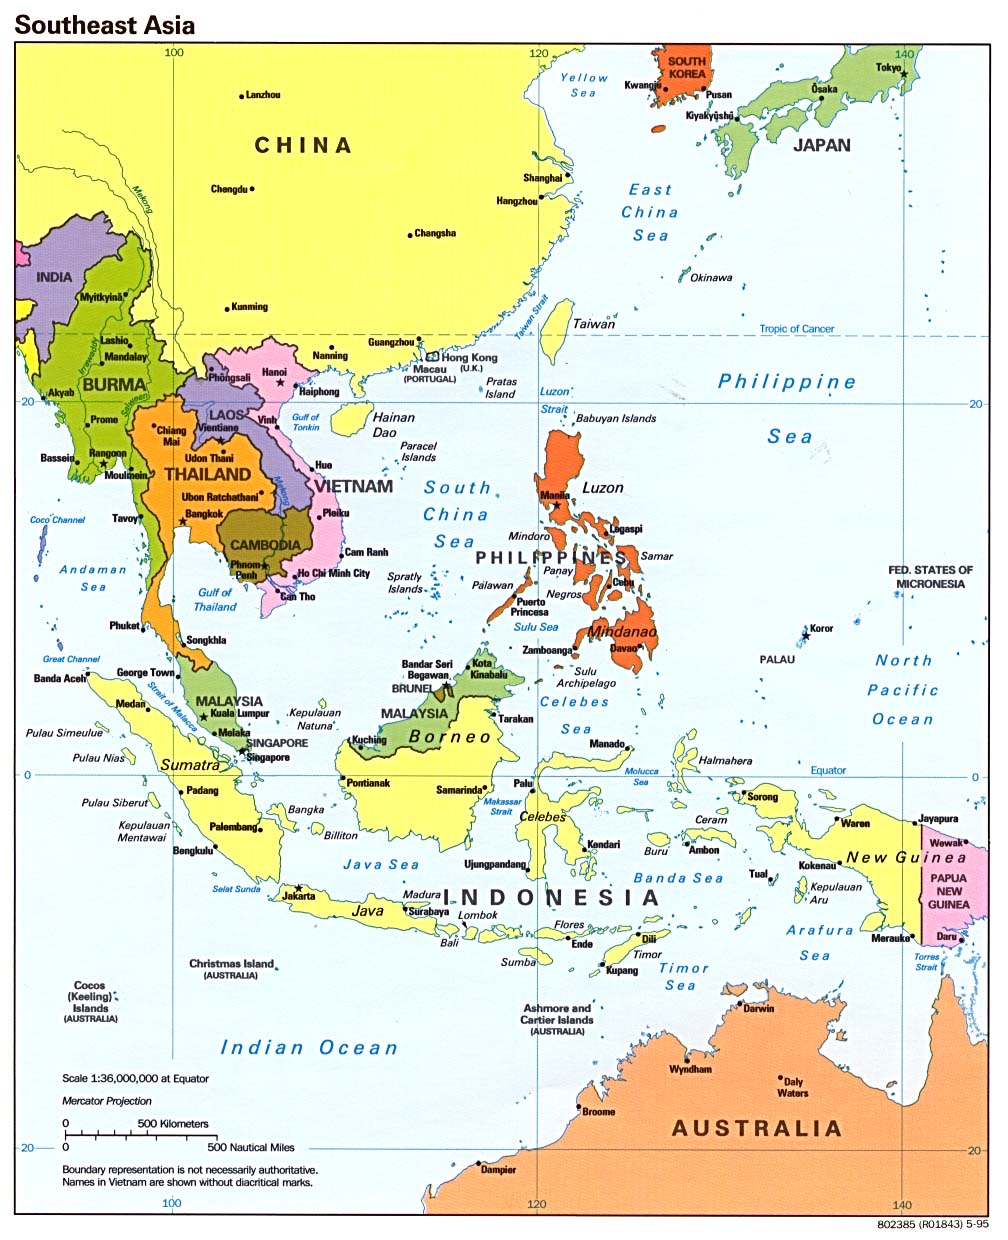
\includegraphics[width=70mm]{map-of-southeast-asia-region.jpg}
 \caption {Map of Southeast Asia region}
      \end{figure}

  As explained in the introduction, sea level rise is a natural phenomenon that has been taking place for thousands of years. Woodroffe (1993) considers a series of unpublished studies on coastal and lowland river plains in Southeast Asia and northern Australia that were a product of the International Geological Correlation Programme Project 274 Coastal Evolution in the Quaternary meeting in Ipoh, Malaysia, which took place in 1989. These studies focus on the evolution of the continental shelves during the Quaternary, 2.6 million years from before present, in the Cenozoic era. The extensive low-gradient continental shelves are exposed as the Sunda platform and Sahul shelf during periods of low sea level. The studies show how evolution in the Quaternary was as a result sea-level change in the region as well as environmental changes, which influenced sediment supply and alluviation. 

\begin{figure}
\centering
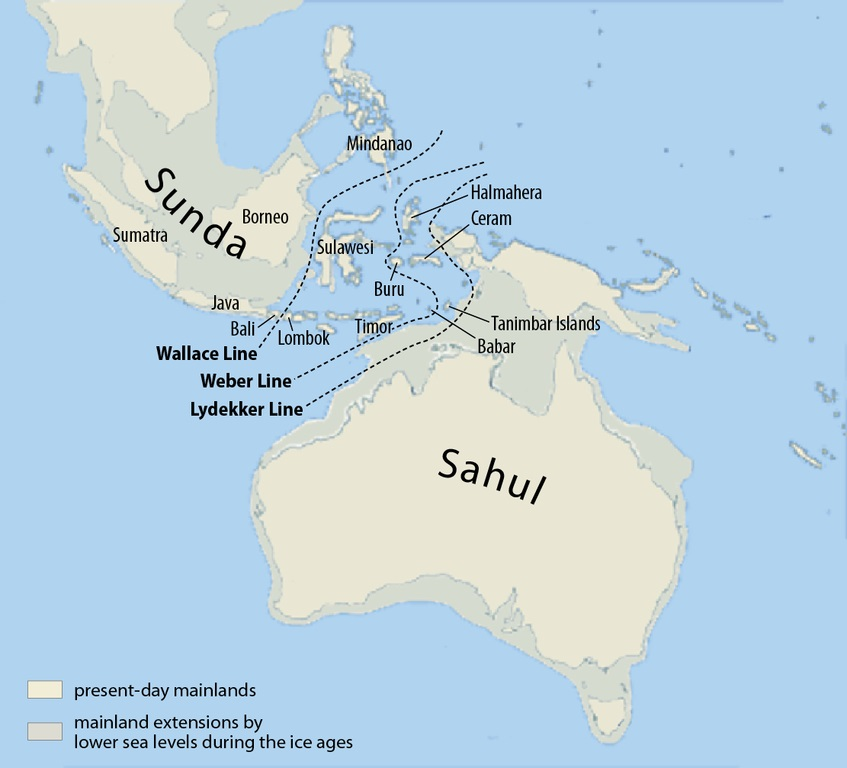
\includegraphics[width=70mm]{Map-of-Sunda-and-Sahul.jpg}
 \caption {The Sunda platform and Sahul shelf, which were exposed during glacial periods in the Cenozoic era.}
\end{figure}

  Woodroffe (1993)\footnote{need to cite properly} considers a series of unpublished studies on coastal and lowland river plains in Southeast Asia and northern Australia that were a produce of the International Geological Correlation Programme Project 274 Coastal Evolution in the Quaternary meeting in Ipoh, Malaysia, which took place in 1989. These studies focus on the evolution of the continental shelves during the Quaternary, 2.6 million years from before present, in the Cenozoic era. The extensive low-gradient continental shelves are exposed as the Sunda platform and Sahul shelf during periods of low sea level. The studies show how evolution in the Quaternary was as a result sea-level change in the region as well as environmental changes, which influenced sediment supply and alluviation.

\begin{figure}
\centering
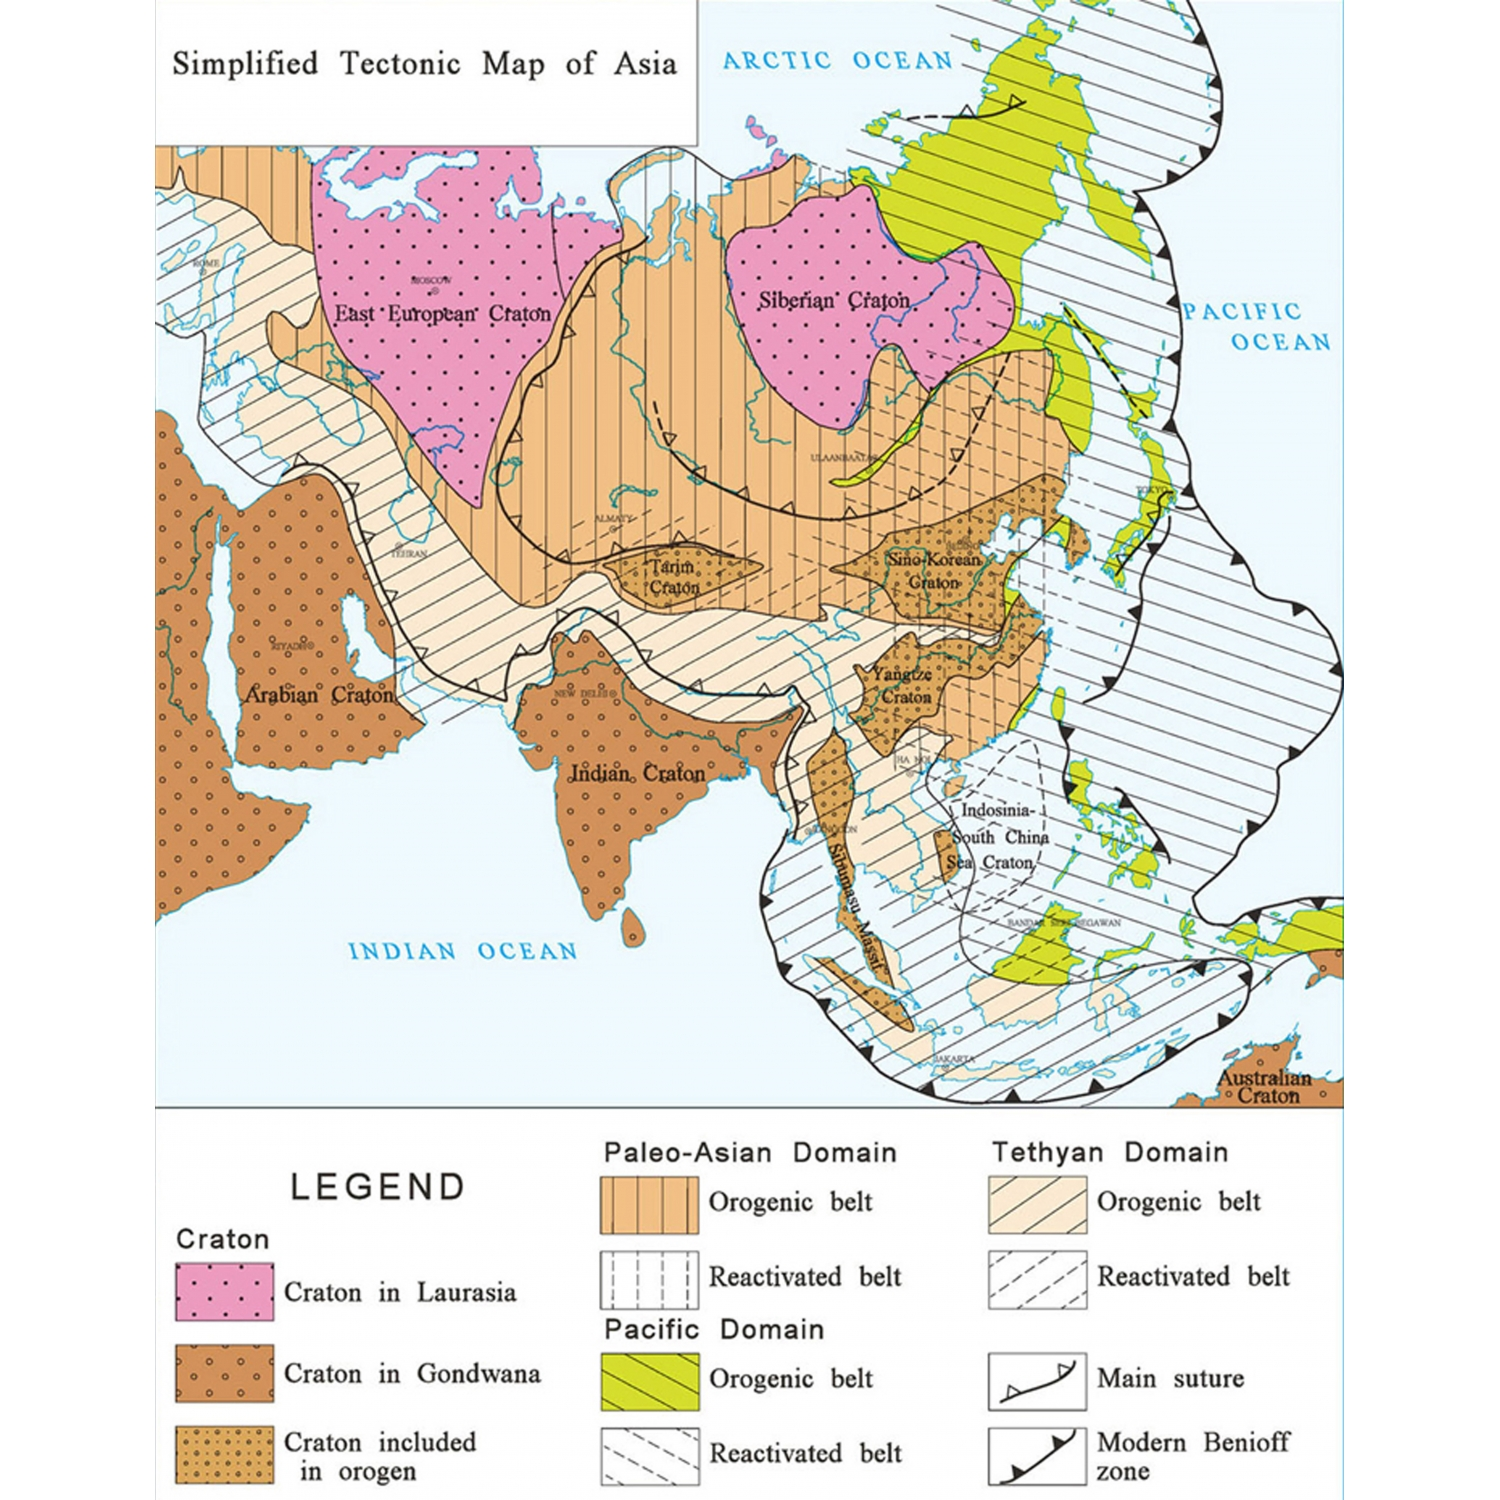
\includegraphics[width=90mm]{geology_southeast_asia.jpg}
\caption{Geology of Southeast Asia.}
\label{fig:SE_asia_geology}
\end{figure}



\subsection{Sea Level Change}
  The sea levels of the Earth shows an overall increase trend particularly after the industrialization. Ocean temperature increases as well which leads to ocean expansion. Globally averaged trend toward rising sea levels makes greater complexities. Regional effects cause sea levels to increase on some parts of the planet, decrease on others, and even to remain relatively flat in a flew places, including, in recent decades, on the California coast. Thermal expansion of seawater can be the product of regional phenomena, such as El Nino, the periodic warming of the eastern tropical Pacific. Temperatures are increasing, leading to ocean expansion.
  
Although sea levels have always fluctuated with changes in global temperature, sea level in Southeast Asia has changed rapidly over the course of  250,000 years (Voris, 2000). A study estimates and indicates that  the areas of exposed land in the Indo-Australian region during periods of the Pleistocene, when sea levels were below present levels, by producing a series of maps. The sea level changes are associated with glaciation that has taken place over the past 250,000 years BP. In this 250,000 year time frame there has been a 120 m sea level change.


\subsection{Isostasy}
  Woodroffe (1993) explains that during the Quaternary, the volumes of oceans increased with melting glaciers and declined with increasing glaciation. The rate of glacial melting slowed dramatically around 6000 years ago. However, there are ongoing isostatic adjustments that are a result of changes in ice load (glacio-isostasy) and changes in the load of water (hydro isostasy), two different factors. 
  
  Isostasy is a naturally occurring process that restores equilibrium between the Earth's crust and the mantle it floats on (Figure~\ref{fig:isostasy}). The mantle is composed of layers with varying densities, two of which are the lithosphere (crust and upper mantle) and the asthenosphere (below lithosphere and flows like asphalt). The process of isostasy demonstrates how subsidence and sea level rise are related. Subsidence occurs when the Earth's surface sinks due to either a geological or human-induced cause. Isostatic sea level change takes place as a result of a load (i.e. ice or water) changes on Earth's crust.

\begin{figure}
\centering
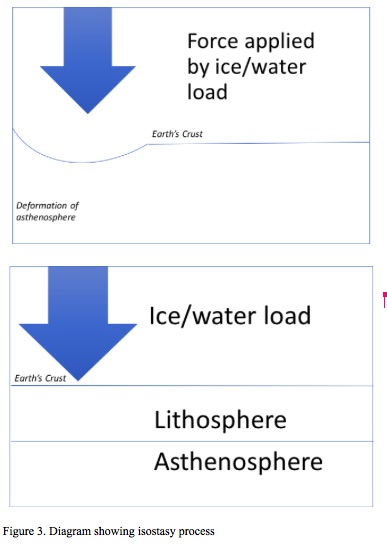
\includegraphics[width=90mm]{IsostasyDiagram.jpg}
\caption {Diagram showing Isostasy Process}
\label{fig:isostasy}
\end{figure}


  The change in load alters the shape of the asthenosphere because it is the weaker layer that is easier to deform. Isostatic sea level change occurs locally, for example when glaciers sit on the Earth�s crust, a gravitational force pulls the glaciers downwards, causing the lithosphere to dip in response to the force in that particular are. The dipping or bulging of the asthenosphere is the subsidence. Since the asthenosphere is viscous, or has a high resistance to flow, the force being applied to the lithosphere by glaciers of water for example, causes it to change its form. The adjustment of the lithosphere in response to the stress being applied is the isostatic adjustment and is possible due to the flowing layer under the lithosphere. The Earth�s crust attempts to reach an equilibrium with the mantle it is floating on. Since the area of the Earth's surface sinks when subsidence occurs, the sea level increases. 

 \section{Groundwater Extraction}
 \subsection{Groundwater}
   Groundwater exists in the multitude of small spaces found within permeable layers of rock and sediment called aquifers. Many aquifers are porous rock covered by soil. Because water can easily flow in and out of such aquifers, they are called unconfined aquifers. In contrast, some aquifers are surrounded by a layer of impermeable rock or clay. These aquifers are called confined aquifers because the impermeable, or confining layer impedes water flow to or from the aquifer. The uppermost level at which the water in a given area fully saturates the rock or soil is called the water table. The water table is therefore the surface of the groundwater in an area.
   
  Challenges posed by groundwater as a resource to humans are connected to both natural events and in Southeast Asia can be caused by natural events and anthropogenic activities. The main problems caused by natural causes affect the quality of groundwater in the arid and semi-arid areas, especially in the central part of Asia. Global climate change made the diversified the hydrogeological conditions in both inland and coastal areas of Asia. Problems caused by human action are groundwater overexploitation and related land subsidence, seawater intrusion and groundwater contamination. Those problems have increased rapidly over the last 20 years. 
  
    Water from precipitation can percolate through the soil and work its way into an aquifer. This input process is known as groundwater recharge. If water falls on land that contains a confined aquifer, however, it cannot penetrate the impermeable layer of rock. Therefore, a confined aquifer cannot be recharged unless the impermeable layer has an opening at the land's surface that can serve as a recharge area. 
    
\section{A Case Study:Mekong Delta}

The most extensive coastal lowland is the lower Mekong basin, which encompasses most of the Cambodia and Southern Vietnam. Mainland SE Asia is drained by five major river systems, which from west to east are the Irrawaddy, Salween, Chao Phraya, Mekong and Red rivers. The Irrawaddy , Salween and Mekong rivers are the three largest systems and their all originated from the plateau of Tibet. 

  Scientific research conducted on sea level rise in the Mekong Delta demonstrate that increased sea level rise will negatively impact rice production. Over the past three decades, the delta has undergone various changes to its hydrology (i.e. canals and sluices) in order to improve agricultural production, specifically rice production. In 2000, 78\% of the land in the delta was being used for rice production and since 1997, rice production in the delta has accounted for 50\% of rice production in Vietnam. As is characteristic of most deltas, most of the land of the Mekong Delta is only slightly above sea level. The major flood of September/October 2000 is one example of the devastating impact of flooding in the Mekong Delta caused by the Mekong River as it lead to large losses in the agricultural sector. Wassmann et al. (2004) focus on the flooding period of the Mekong Delta between the months August and November. They use a hydraulic model, �Vietnam River Systems and Plains� (VRSAP) to evaluate future changes in the Mekong Delta. In general, the water levels in the Mekong Delta are influenced by water discharge of the Mekong River, tidal variations in the South China Sea and the Gulf of Thailand. 

\begin{figure}
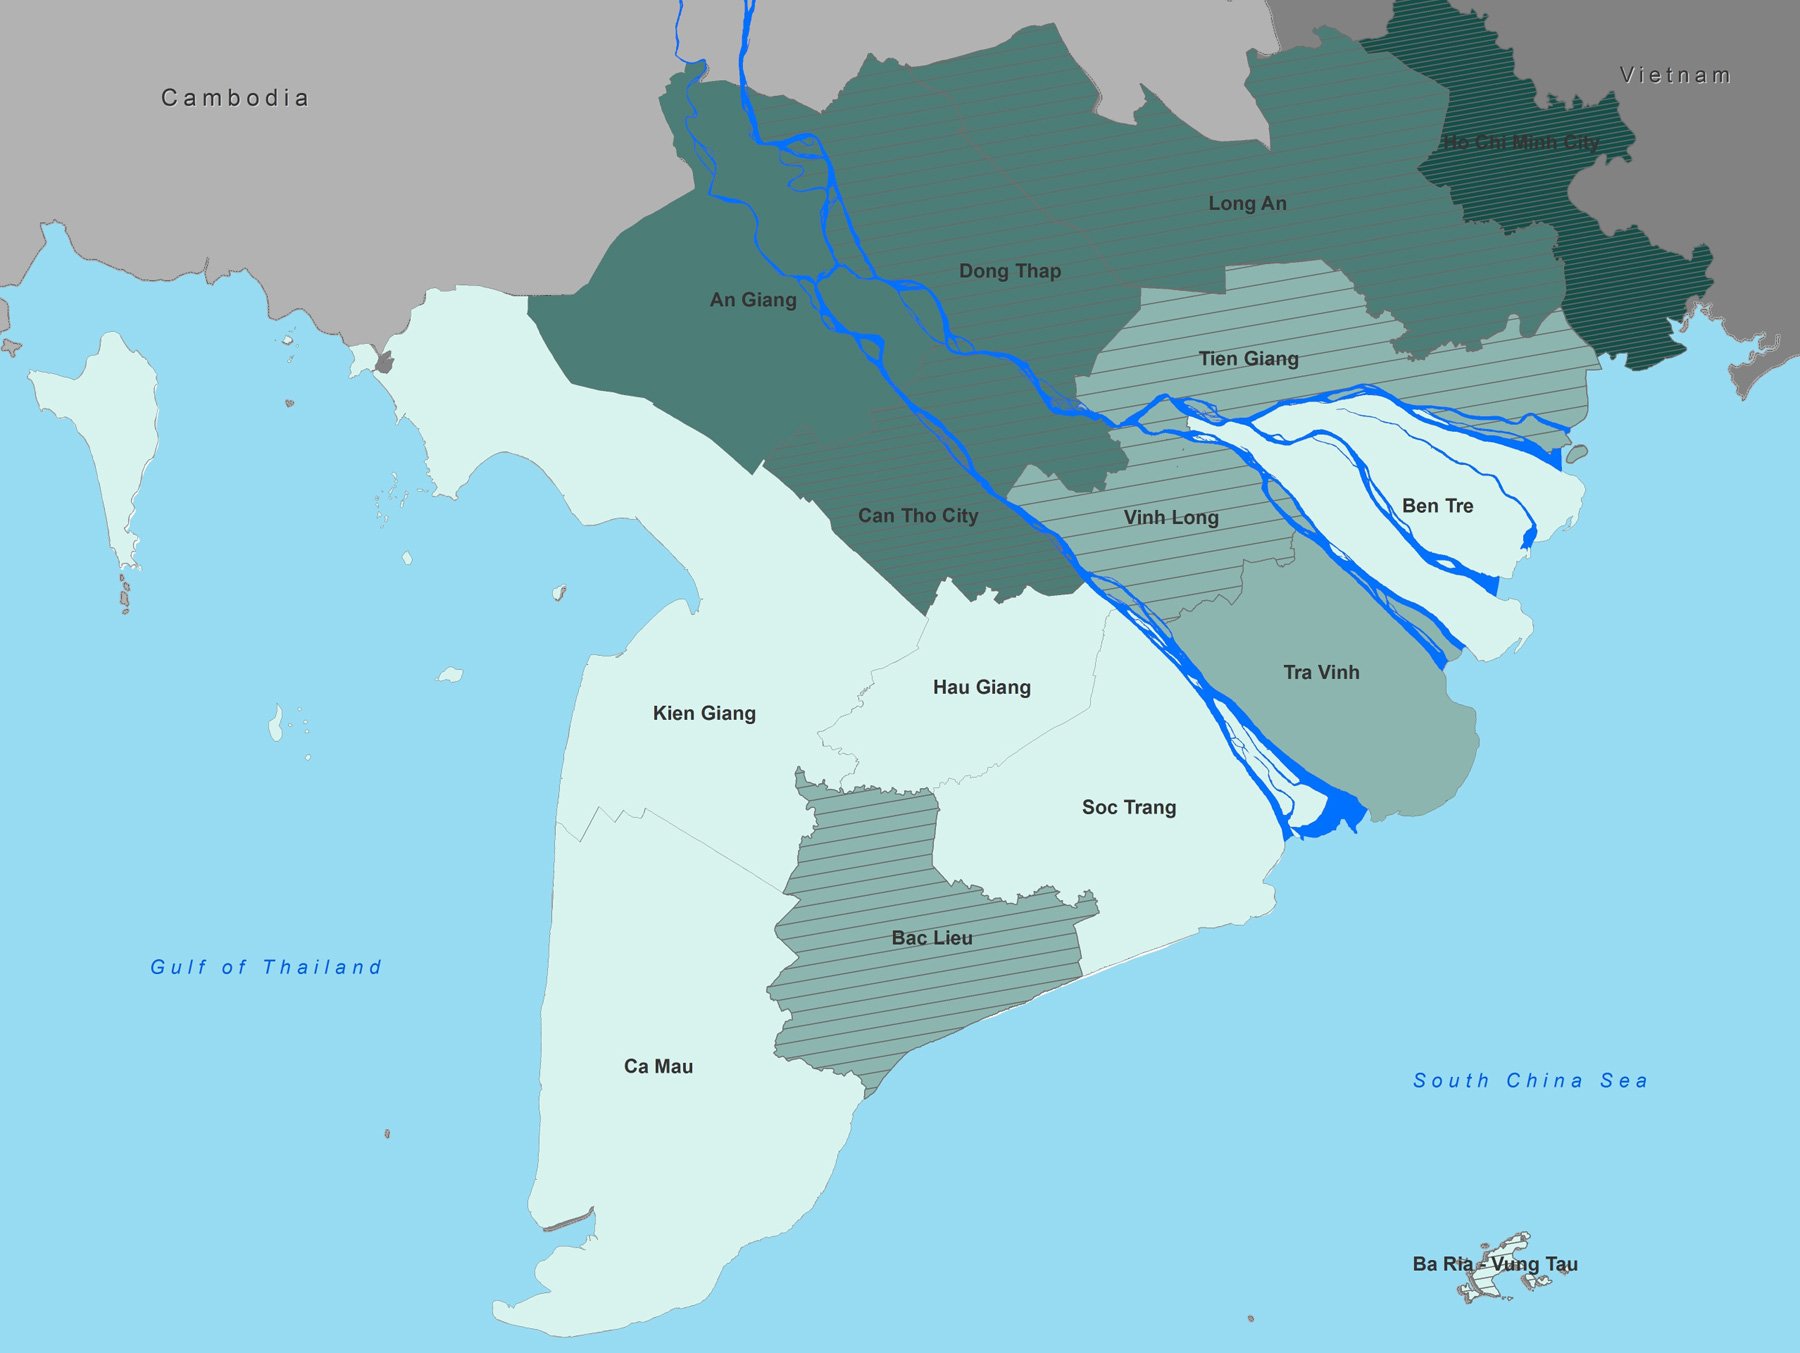
\includegraphics[width=90mm]{mekong-delta-vietnam-maps.jpg}
\caption{Map showing relative locations of the Vietnamese Mekong Delta, the Mekong River, the South China Sea and the Gulf of Thailand.}
\end{figure}

  High upstream discharge and heavy rainfall in September and October increase the likelihood of flooding in the Mekong Delta and high tidal levels are recorded in January. In terms of the impact of flooding, the upper part of the Mekong Delta is characterized as a deeply flooded area, mostly affected by river discharge, and the lower part of it is characterized as a shallow flooded area, which is largely as a result of tide. The scenarios presented by Wassmann et al. (2004) correspond to the medium-term (year 2030) and long-term projections  of the original Business-as-Usual scenario provided by the Intergovernmental Panel of Climate Change (IPCC, 1990). The researchers project a 20cm sea level rise in as early as 2040 and latest by 2100. The construction of water control systems such as hydro-dams or an increase in water withdrawal could possibly exacerbate the conditions in the Mekong Delta when sea level rises, which will be discussed later in this chapter.

\subsection{Geographical Context of Mekong Delta}
  The origin of the Mekong river lies 5,000 meters above sea level, situated high on the Tibetan plateau. From there the river runs through China's Qinghai and Yunnan provinces, where it is called the Lancang River. The name changes to ''Mekong'' when it gets to the other SE Asia nation: Myanmar, Lao, Thailand, Cambodia and eventually settled at the Mekong Delta in Vietnam. Under natural conditions, delta subsidence is offset by deposition of fluvial sediment, particularly during flood overspill of river banks. Sediment reaching the coastal environment can accumulate in a seaward progradation of the shorefront and/or delta front. [1] The Mekong Delta region displays a variety of physical landscapes, but is dominated by flat floodplains in the south, with a few hills in the north and west. The diversity of terrain was largely the product of tectonic uplift and folding brought about by the collision of the Indian and Eurasian tectonic plates about 50 million years ago. The soil of the lower Delta consist mainly of sediment from the Mekong and its tributaries, deposited over thousand of years as the river changed its course.
  
  Understanding the geologic history of the upper Mekong basin is crucial for examining the effects of dam construction. Most of the Vietnam Mekong Delta is only slightly above the mean sea level and both tidal flooding from the Mekong River and saltwater intrusion negatively affect on the agricultural sector (Wassmann et al., 2004). 

  Stratigraphy is a terminology referring to the study of strata (rock layers) and stratification ( the formation of strata in rock). In this case, the stratigraphic formation looks at sedimentary and layered volcanic rocks of the Mekong river delta, which helps to understand its geologic evolution as well as the rapid coastal changes.The Mekong Delta region displays a variety of physical landscapes, but is dominated by flat floodplains in the south, with a few hills in the north and west. The diversity of terrain was largely the product of tectonic uplift and folding brought about by the collision of the Indian and Eurasian tectonic plates about 50 million years ago. The soil of the lower Delta consist mainly of sediment from the Mekong and its tributaries, deposited over thousand of years as the river changed its course. Under natural conditions, delta subsidence is offset by deposition of fluvial sediment, particularly during flood overspill of river banks. Sediment reaching the coastal environment can accumulate [a growth of river delta further out into the sea over time and] form a seaward propradation of the shorefront. This happens when the mass amount of sediment is carried from the river into the ocean ( and disposed at the estuary) and the rate of such sediment piling up is greater than the volume of the delta that is lost. Subsidence, sea-level rise and coastal erosion can all potentially contribute to the lost of the delta. The difference between delta and normal landscape.. And its implication and legacy on the differences.
  
  The morden Mekong Delta was initiated during the local sea level still-stand about 7,500 years ago (Bird at al., 2010; Hanebuth et al., 2012). Since the middle Holocene (around 7,500 years ago), the delta has prograded more than 220 km from Cambodia eastward into the East Sea at a long-term mean rate of a~30 m yr-1. This progradation has buried earlier phases of the delta beneath later subaerial deltaic deposits, thus becoming the foundation for delta development. Research indicates that the the current coastal zone on the shelf was formed only in the past 1,000 years. The characteristic of this delta evolution model is different from those of other large river delta systems on the East Asian Margins as as the Yangtze, the Pearl, as well as the Red Rivers. Due to it young age, the deposit of Mekong delta is relatively unstable and constantly creating new shoreline and moving steward.Whereas the paths of along-shelf transport and locations of distal accumulations for the other deltas have been relatively unchanged for the past 7,000 years (J.P Liu at al, 2009, in press).\footnote{fix citation}
  
\subsection{Shoreline and Coastal Erosion}

  Throughout the past 7,500 years, the Mekong River mouth has expanded seaward over 220 km and built a 61,000 km2 delta in total. Based on the size and age of the Mekong Delta, the long-term average shoreline growth has been 30 meters per year. However, the delta has been experiencing large-scale shoreline erosion and land loss in the past decade. 
  
Due to gradually increasing ground water extraction over the past 25 years, on average the Mekong Delta has subsided roughly about 18 cm, with some areas sinking more than 30 cm (Erban et al., 2014; Minderhoud et al., 2017.). Additionally, the total coverage of mangrove forests on the Mekong delta coastal zone decreased by 50\% between 2965 and 2001, with most of these forests destroyed after 1995 (Thu and Populus, 2007).\footnote{fix citation} 

\subsection{Socio-economic Considerations}

  Over the past few decades, water resource development literature has presented the inevitability of a global water crisis. These projections stem from the increasing concern over the limited fresh water resources available to humans.  The strategies that have been proposed by various actors such as the global water industry, the United Nations, government representatives, policy makers and scientific experts have focused on �cooperation� in the `international community.' Sneddon and Fox (2006) illuminate how these negotiations obscure the extent to which states, nonstate actors and river basins construct `transnational'�' river basins through institutional and material processes.
  
Sneddon and Fox (2006)\footnote{fix citation} offer an analysis of how transboundary river basins, like the Mekong River, that encompass various sovereign states, are managed through institutional arrangements, pointing to the limitations of constructing natural resources through legal arrangements or geopolitical framings. With a focus on the Mekong, they offer a critical hydropolitics that brings together political and human-environmental geography to reveal how geopolitical constructions simplify connections and hide environmental conflicts. 

  In 1957, the Committee for the Coordination of Investigations in the Lower Mekong Basin was created under the support of the United Nations Development Program (UNDP). Over the subsequent 15 years the Committee collected hydrologic data necessary for the construction of large scale mainstream hydroelectric dams and oversaw tributary projects in the national territories of the Lower Basin states (Laos, Thailand, Cambodia, and Vietnam).
  
  During the armed struggle between Vietnam and the United States between mid-1960s to early 1970s, the Mekong served as a symbol of cooperation in Cold War geopolitics. The symbol of peace was to be achieved through cooperation of the four nation states that are traversed by the Mekong. Sneddon and Fox (2006) explain that the United States led cooperative development of the Mekong following the creation of the Mekong Delta through the work of United States Reclamation and Army Corps of Engineers. However, they emphasize that the United States was using its involvement in the Mekong to further a geopolitical strategy to provide aid to economic development projects in the region (i.e. Thailand) as material and ideological counterpoints to socialism. The aid-driven relationship between Thailand and the United States resulted in the relegation of disproportionate decision-making power to the Thai government when it came to Mekong matters.
  
  
Although the United States continued to support Thailand financially and militarily throughout the 1960s and 1970s, when the US Forces were withdrawn from Vietnam in the mid-1970s, there was a complimentary abandonment of the Mekong as a geopolitical strategy. Three years after the ascension of the Khmer Rouge regime in Cambodia, in 1978, the Mekong Committee became the Interim Mekong Committee (IMC). Following the civil war in Cambodia in 1991, the government began to view the Mekong as a driving force for rapid economic development because of its hydroelectric power and water storage capacity for irrigation schemes. It is clear how government and trans-national approaches to the management of water resources in the Mekong were cleary state-centrist. 

\subsection{Anthropogenic Environmental Challenges}

\subsubsection{Arsenic Contamination}

How are the geographical features of the Mekong Delta providing resources to humans and furthermore, what elements of their formation pose challenges to how Vietnamese people will interact with these features in the future?

  Erban et al. (2013)\footnote{fix citation} investigate the challenges being posed by the overexploitation of aquifers in South and Southeast Asia, with a specific focus on Vietnam. Their research focus is a large (>1,000 km2)  area of the Mekong Delta in Vietnam. Arsenic in groundwater continues to threaten human health in this region. It is a colorless, odorless, and tasteless poison that is toxic to humans if they are exposed to it over a long period of time (Ravenscroft, year)\footnote{fix citation}. The poison occurs most commonly in sands deposited by large rivers, with the worst cases recorded in the tropical basins of Asia. Arsenic-contaminated groundwater is found in the unconsolidated sediments and sedimentary, igneous and metamorphic rock which age in range from thousands of years to billions. In most cases, high levels of arsenic in the groundwater also means there is arsenic in the soils. The effects of arsenic in groundwater is both additive and cumulative because plants can absorb arsenic through the roots. The subsistence rice economies of Asia, whereby rice is irrigated with arsenic-contaminated water, present the worst cases. The deep aquifers are presumed to be sources of pathogen- and arsenic-free water. 

\subsubsection{Historical Context}

  Pliocene-Miocene-age aquifers in the Mekong Delta are contaminated at depths of 200-500 m and they have been heavily exploited. Generally, seven main aquifers are heavily pumped in the Mekong Delta, varying from the Pliocene to the Miocene age. The Division for Geological Mapping for the South of Vietnam, who used a combination of scientific techniques  (i.e. mud logging of drill cuttings), determined the delineation of aquifers and their ages, used by Erban et al.\footnote{fix citation} in this work. Pumping wells is a process that existed in Vietnam since the 1900s, but became more common after the 1980s. The dissolved concentrations of arsenic are highest near the surface, closer to the Mekong river and its tributaries, reducing greatly with distance. Extreme arsenic concentrations are found in numerous hot spot regions. Erban et al. found that deep wells located in the focus areas of the research in the Mekong area showed more contamination than in other parts of Southeast Asia.
  
  An analysis of satellite-based radar images recorded from 2007 to 2010 shows how intensive groundwater extraction has caused land subsidence of up to 3cm/year. Furthermore, transient 3D aquifer simulations show similar subsidence rates with a total subsidence of up to 27 cm since 1988.  Erban et al. (2013)\footnote{fix citation} propose a causal mechanism that explains the long-term effect of groundwater extraction on interbedded clays. The groundwater extraction causes these interbedded clays to compact and expel water containing dissolved arsenic or arsenic-mobilizing solutes, examples being dissolved organic carbon and competing ions, into deep aquifers over decades.
  
  The subsequent threat is that deep, untreated groundwater in the Mekong Delta Region will no longer be a safe source of drinking water. The pumping-induced clay compaction was measured as land subsidence. Erban et al. present a conceptual model that explains the vertical distribution of arsenic in the Mekong Delta according to how it developed historically. Starting in the Miocene age and tracking to the present, the researchers explain how fresh clays rich in arsenic and organic compound were deposited widely. The slow diffusion out of contaminated pores and dissolution of the solid-phase arsenic supply allowed for a continuous deep arsenic load in deep clays. Recently, the overpumping of low-arsenic, deep aquifers resulted in causing water carrying arsenic-mobilizing solutes to be squeezed out of the deadflow storage of clays to neighbouring aquifers. 


\subsection {Dam Construction}
  In the past decades, hydroelectric dam developments has been growing steadily in Asia. Although hydroelectricity is considered as a renewable energy, there are numerous negative impacts associated with large dam construction. Researches have revealed some common effects of dams which include:
  
  The modification of flow regimes both upstream and downstream (Williams and Wolman, 1984; Knighton, 1988; Iba`n ?ez et al., 1996; Batalla et al., 2004)\footnote{fix citation}, The trapping of sediment in reservoirs and disruption of sediment transport downstream (Phillips, 2001, 2003, 2004; Vo ?ro ?smarty et al., 2003; Walling and Fang, 2003)\footnote{fix citation}. 
  
The reduction of biodiversity due to the flooding of habitat, isolation of animal populations and blocking of migration routes (Gehrke et al., 1995; Kingsford, 2000;\footnote{fix citation} Bunn and Arthington, 2002)

In estuarial areas, changes in downstream riparian vegetation and salt wedge dynamics (Wolanski et al., 1996; Friedman et al., 1998).\footnote{fix citation}


The Mekong River delta, similarly, is undergoing some of the geologic and environmental challenges. Given the fact that Mekong river started in Himalayas and goes through six countries, different nations are developing different parts of the river individually. Oftentime, concerns have been raised regarding the mismanagements of the upper stream which could potentially lead to lost of lands as well as livelihood for lower Mekong basin residents. 

For example, China has been developing a series of eight large scale dams in upper stream of Mekong. Whereas sediment supplies are critically crucial for river deltas to maintain the shorelines and balance annual subsidence lost to the ocean. This series of dmas, termed as the Mekong Cascade, will be constructed over a 750k length in the upper basin of the Mekong River in Yunnan, over a total gradient change of 800m (Plinston and He, 1999)\footnote{fix citation}. 

\subsection{Mitigation}

  Kench et al. (2015)\footnote{fix citation} conducted research on low-lying coral reef islands, such as the Maldives in the Indian Ocean, to demonstrate how coral reefs adapt to sea level rise. A combination of various factors, such as low elevation, small area, sensitivity to variations in boundary conditions, cause the stability of these areas to be of special global concern. The researchers focus on the morphological responses of of islands to recent sea level rise by analyzing a centennial-scale record of physical changes in the islands of Funafuti Atoll, Tuvalu, located in the central Pacific Ocean. For the past 60 years, the researchers found that the majority of islands increased in area in response to sea level rise instead of experiencing widespread erosion. An explanation they offer for why these islands increased is the island accretion through generation of new gravel during cyclonic events that have transported to the island shoreline. Their results present that island can persist on reefs when the rate of sea level rise is 5 mm/yr, however as sea level is projected to rise by 1.2 metres by 2100, it will be uncertain whether or not islands will be able to continue to maintain this dynamic adjustment. The challenge posed by these higher rates of change is the development of flexible adaptation strategies that recognize the urgent circumstances of island margins. Their research provides a platform for a discussion on how governments can implement adaptive strategies that use biomimicry. The accretion of gravel and sand in low-lying coral reef islands is a natural process. However, humans can also add gravel to reef islands that are experiencing erosion or submergence as a result of sea level rise. The challenges being posed by sea level rise in the Mekong Delta can be tackled through this approach. To be more specific, conducting research on how accretion of soil, or other natural substances occurs in deltas, can be useful for scientists and researchers who may be able to propose ways humans can  replicate these processes. 

\subsection{Conclusion}

???

Introduction to powers of exclusion: land dilemmas in Southeast Asia
D Hall, P Hirsch, TM Li
National University of Singapore Press and University of Hawaii Press	457	2011
Development dilemmas in rural Thailand.
P Hirsch
Development dilemmas in rural Thailand.	203	1990
The politics of environment in Southeast Asia: resources and resistance
P Hirsch, C Warren
Psychology Press	150	1998
River basin closure: Processes, implications and responses
F Molle, P Wester, P Hirsch
Agricultural Water Management 97 (4), 569-577	130	2010
National interests and transboundary water governance in the Mekong
P Hirsch, KM Jensen, B Boer, N Carrard, S FitzGerald, R Lyster
Australian Mekong Resource Centre, in collaboration with Danish …	128	2006
Contemporary politics of environment in Thailand
P Hirsch, L Lohmann
Asian Survey 29 (4), 439-451	112	1989
Resources, nations and indigenous peoples
R Howitt, J Connell, P Hirsch
Oxford University Press, Melbourne	111	1996
Seeing forests for trees
P Hirsch
Environment and Environmentalism in Thailand	107	1997
Globalisation, regionalisation and local voices: The Asian Development Bank and rescaled politics of environment in the Mekong region
P Hirsch
Singapore Journal of Tropical Geography 22 (3), 237-251	104	2001
Forests, forest reserve, and forest land in Thailand
P Hirsch
Geographical Journal, 166-174	101	1990
Negotiating local livelihoods: scales of conflict in the Se San River Basin
P Hirsch, A Wyatt
Asia Pacific Viewpoint 45 (1), 51-68	92	2004
Political economy of environment in Thailand
P Hirsch
Journal of Contemporary Asia Publishers	88	1993
Resources, nations, and indigenous peoples: case studies from Australasia, Melanesia, and Southeast Asia
R Howitt, J Connell, P Hirsch
Oxford University Press, USA	83	1996
Deforestation and development in Thailand
P Hirsch
Singapore Journal of Tropical Geography 8 (2), 129-138	82	1988
The changing political dynamics of dam building on the Mekong
P Hirsch
Water Alternatives 3 (2), 312	79	2010
Water governance reform and catchment management in the Mekong region
P Hirsch
The Journal of Environment \& Development 15 (2), 184-201	70	2006
Can SIA empower communities?
C Gagnon, P Hirsch, R Howitt
Environmental Impact Assessment Review 13 (4), 229-253	68	1993
Thailand and the new geopolitics of Southeast Asia: Resource and environmental issues
P Hirsch
Counting the costs: Economic growth and environmental change in Thailand …	62	1995
Natural Resource Management in the Mekong River Basin: Perspectives for Australian Development Cooperation. Final overview report to AusAID. The
P Hirsch, G Cheong, R Gartrell, P Hinton, NV Thinh, F Miller
56	1996
The state in the village: interpreting rural development in Thailand
P Hirsch
Development and Change 20 (1), 35-56
